

\tikzset{every picture/.style={line width=0.75pt}} %set default line width to 0.75pt        

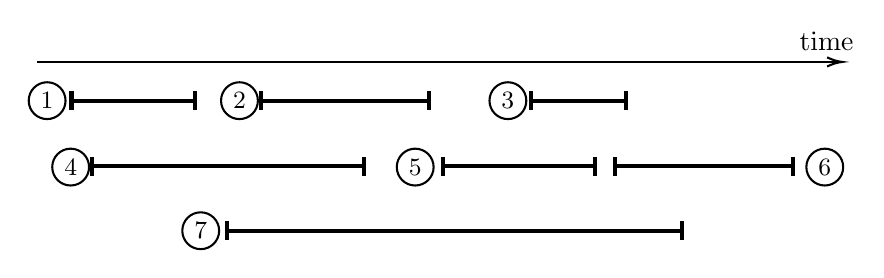
\begin{tikzpicture}[x=0.5pt,y=0.5pt,yscale=-1,xscale=1]
%uncomment if require: \path (0,187); %set diagram left start at 0, and has height of 187

%Straight Lines [id:da9015649955021968] 
\draw    (7,37) -- (587,37) ;
\draw [shift={(589,37)}, rotate = 180] [color={rgb, 255:red, 0; green, 0; blue, 0 }  ][line width=0.75]    (10.93,-3.29) .. controls (6.95,-1.4) and (3.31,-0.3) .. (0,0) .. controls (3.31,0.3) and (6.95,1.4) .. (10.93,3.29)   ;
%Straight Lines [id:da9640237890291299] 
\draw [line width=1.5]    (32,65) -- (121.5,65) ;
\draw [shift={(121.5,65)}, rotate = 180] [color={rgb, 255:red, 0; green, 0; blue, 0 }  ][line width=1.5]    (0,6.71) -- (0,-6.71)   ;
\draw [shift={(32,65)}, rotate = 180] [color={rgb, 255:red, 0; green, 0; blue, 0 }  ][line width=1.5]    (0,6.71) -- (0,-6.71)   ;
%Straight Lines [id:da3355888679808179] 
\draw [line width=1.5]    (169,65) -- (290.5,65) ;
\draw [shift={(290.5,65)}, rotate = 180] [color={rgb, 255:red, 0; green, 0; blue, 0 }  ][line width=1.5]    (0,6.71) -- (0,-6.71)   ;
\draw [shift={(169,65)}, rotate = 180] [color={rgb, 255:red, 0; green, 0; blue, 0 }  ][line width=1.5]    (0,6.71) -- (0,-6.71)   ;
%Straight Lines [id:da09988799250468405] 
\draw [line width=1.5]    (364,65) -- (432.5,65) ;
\draw [shift={(432.5,65)}, rotate = 180] [color={rgb, 255:red, 0; green, 0; blue, 0 }  ][line width=1.5]    (0,6.71) -- (0,-6.71)   ;
\draw [shift={(364,65)}, rotate = 180] [color={rgb, 255:red, 0; green, 0; blue, 0 }  ][line width=1.5]    (0,6.71) -- (0,-6.71)   ;
%Straight Lines [id:da4026459071674142] 
\draw [line width=1.5]    (47,112.5) -- (243.5,112.5) ;
\draw [shift={(243.5,112.5)}, rotate = 180] [color={rgb, 255:red, 0; green, 0; blue, 0 }  ][line width=1.5]    (0,6.71) -- (0,-6.71)   ;
\draw [shift={(47,112.5)}, rotate = 180] [color={rgb, 255:red, 0; green, 0; blue, 0 }  ][line width=1.5]    (0,6.71) -- (0,-6.71)   ;
%Straight Lines [id:da5509115882034084] 
\draw [line width=1.5]    (300.5,112.5) -- (410.5,112.5) ;
\draw [shift={(410.5,112.5)}, rotate = 180] [color={rgb, 255:red, 0; green, 0; blue, 0 }  ][line width=1.5]    (0,6.71) -- (0,-6.71)   ;
\draw [shift={(300.5,112.5)}, rotate = 180] [color={rgb, 255:red, 0; green, 0; blue, 0 }  ][line width=1.5]    (0,6.71) -- (0,-6.71)   ;
%Straight Lines [id:da6271509388583772] 
\draw [line width=1.5]    (425,112.5) -- (553.5,112.5) ;
\draw [shift={(553.5,112.5)}, rotate = 180] [color={rgb, 255:red, 0; green, 0; blue, 0 }  ][line width=1.5]    (0,6.71) -- (0,-6.71)   ;
\draw [shift={(425,112.5)}, rotate = 180] [color={rgb, 255:red, 0; green, 0; blue, 0 }  ][line width=1.5]    (0,6.71) -- (0,-6.71)   ;
%Straight Lines [id:da26802882985941956] 
\draw [line width=1.5]    (144.5,159) -- (473,159) ;
\draw [shift={(473,159)}, rotate = 180] [color={rgb, 255:red, 0; green, 0; blue, 0 }  ][line width=1.5]    (0,6.71) -- (0,-6.71)   ;
\draw [shift={(144.5,159)}, rotate = 180] [color={rgb, 255:red, 0; green, 0; blue, 0 }  ][line width=1.5]    (0,6.71) -- (0,-6.71)   ;

% Text Node
\draw (556,13) node [anchor=north west][inner sep=0.75pt]   [align=left] {time};
% Text Node
\draw    (14.38, 65) circle [x radius= 13.31, y radius= 13.31]   ;
\draw (14.38,65) node  [font=\small] [align=left] {$\displaystyle 1$};
% Text Node
\draw    (153.38, 65) circle [x radius= 13.31, y radius= 13.31]   ;
\draw (153.38,65) node  [font=\small] [align=left] {$\displaystyle 2$};
% Text Node
\draw    (347.38, 65) circle [x radius= 13.31, y radius= 13.31]   ;
\draw (347.38,65) node  [font=\small] [align=left] {$\displaystyle 3$};
% Text Node
\draw    (31.38, 113) circle [x radius= 13.31, y radius= 13.31]   ;
\draw (31.38,113) node  [font=\small] [align=left] {$\displaystyle 4$};
% Text Node
\draw    (280.38, 113) circle [x radius= 13.31, y radius= 13.31]   ;
\draw (280.38,113) node  [font=\small] [align=left] {$\displaystyle 5$};
% Text Node
\draw    (576.38, 113) circle [x radius= 13.31, y radius= 13.31]   ;
\draw (576.38,113) node  [font=\small] [align=left] {$\displaystyle 6$};
% Text Node
\draw    (125.38, 159) circle [x radius= 13.31, y radius= 13.31]   ;
\draw (125.38,159) node  [font=\small] [align=left] {$\displaystyle 7$};


\end{tikzpicture}

